\newSection{HairStep}

%---------------------------------------------------------
\subsection{HairStep Representation}
%---------------------------------------------------------

\begin{frame}[t]{HairStep Representation}
    \textit{HairStep} is defined as $\mathbf{H} = \{\mathbf{O}, \mathbf{D}\}$ for each input image $\mathbf{I} \in \mathbb{R}^{W \times H \times 3}$, where:
    \begin{itemize}
        \item $\mathbf{O} \in \mathbb{R}^{W \times H \times 3}$ is the \emph{Strand Map}.
        \item $\mathbf{D} \in \mathbb{R}^{W \times H \times 1}$ is the \emph{Depth Map}.
    \end{itemize}

    \begin{figure}[t]
        \centering
        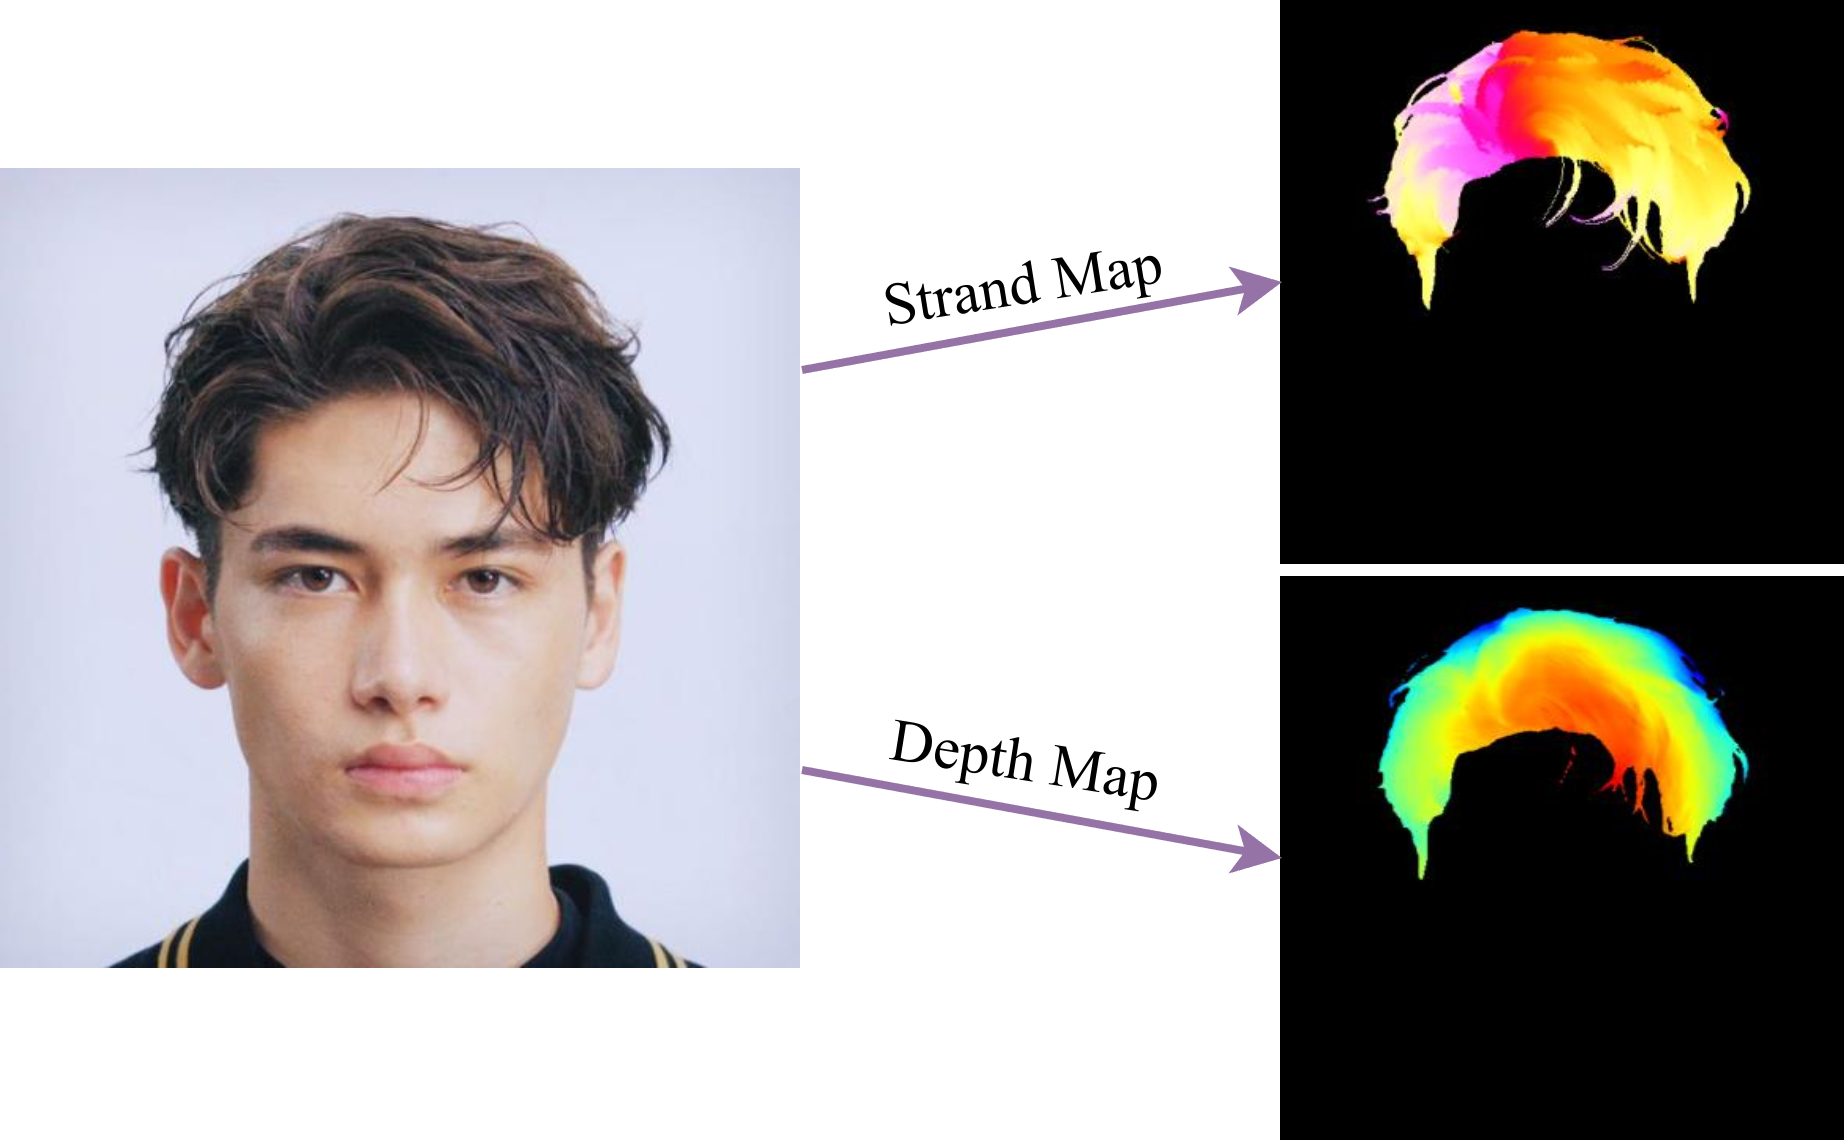
\includegraphics[width=0.45\textwidth]{assets/figures/method/hairstep.png}
        \caption{Example of the HairStep representation.}
        \label{fig:hairstep_rep}
    \end{figure}
\end{frame}

%---------------------------------------------------------
\begin{frame}[t]{HairStep Representation -- Strand Map}
    \textit{Strand Map} $\mathbf{O} \in \mathbb{R}^{W \times H \times 3}$ is defined at each pixel $x$ as
    \begin{equation}
        \mathbf{O}(x) = \bigl(\mathbf{M}(x),\; \tfrac{\mathbf{O}_{\mathrm{2D}}(x)}{2} + 0.5\bigr),
        \label{eq:strand_map}
    \end{equation}
    where:
    \begin{itemize}
        \item $\mathbf{M}(x) \in \{0, 1\}$ is a hair mask (1 denotes hair, 0 denotes background).
        \item $\mathbf{O}_{\mathrm{2D}}(x) \in \mathbb{R}^2$ is the unit vector of 2D hair-growth orientation.
    \end{itemize}
    
    \begin{figure}[t]
        \centering
        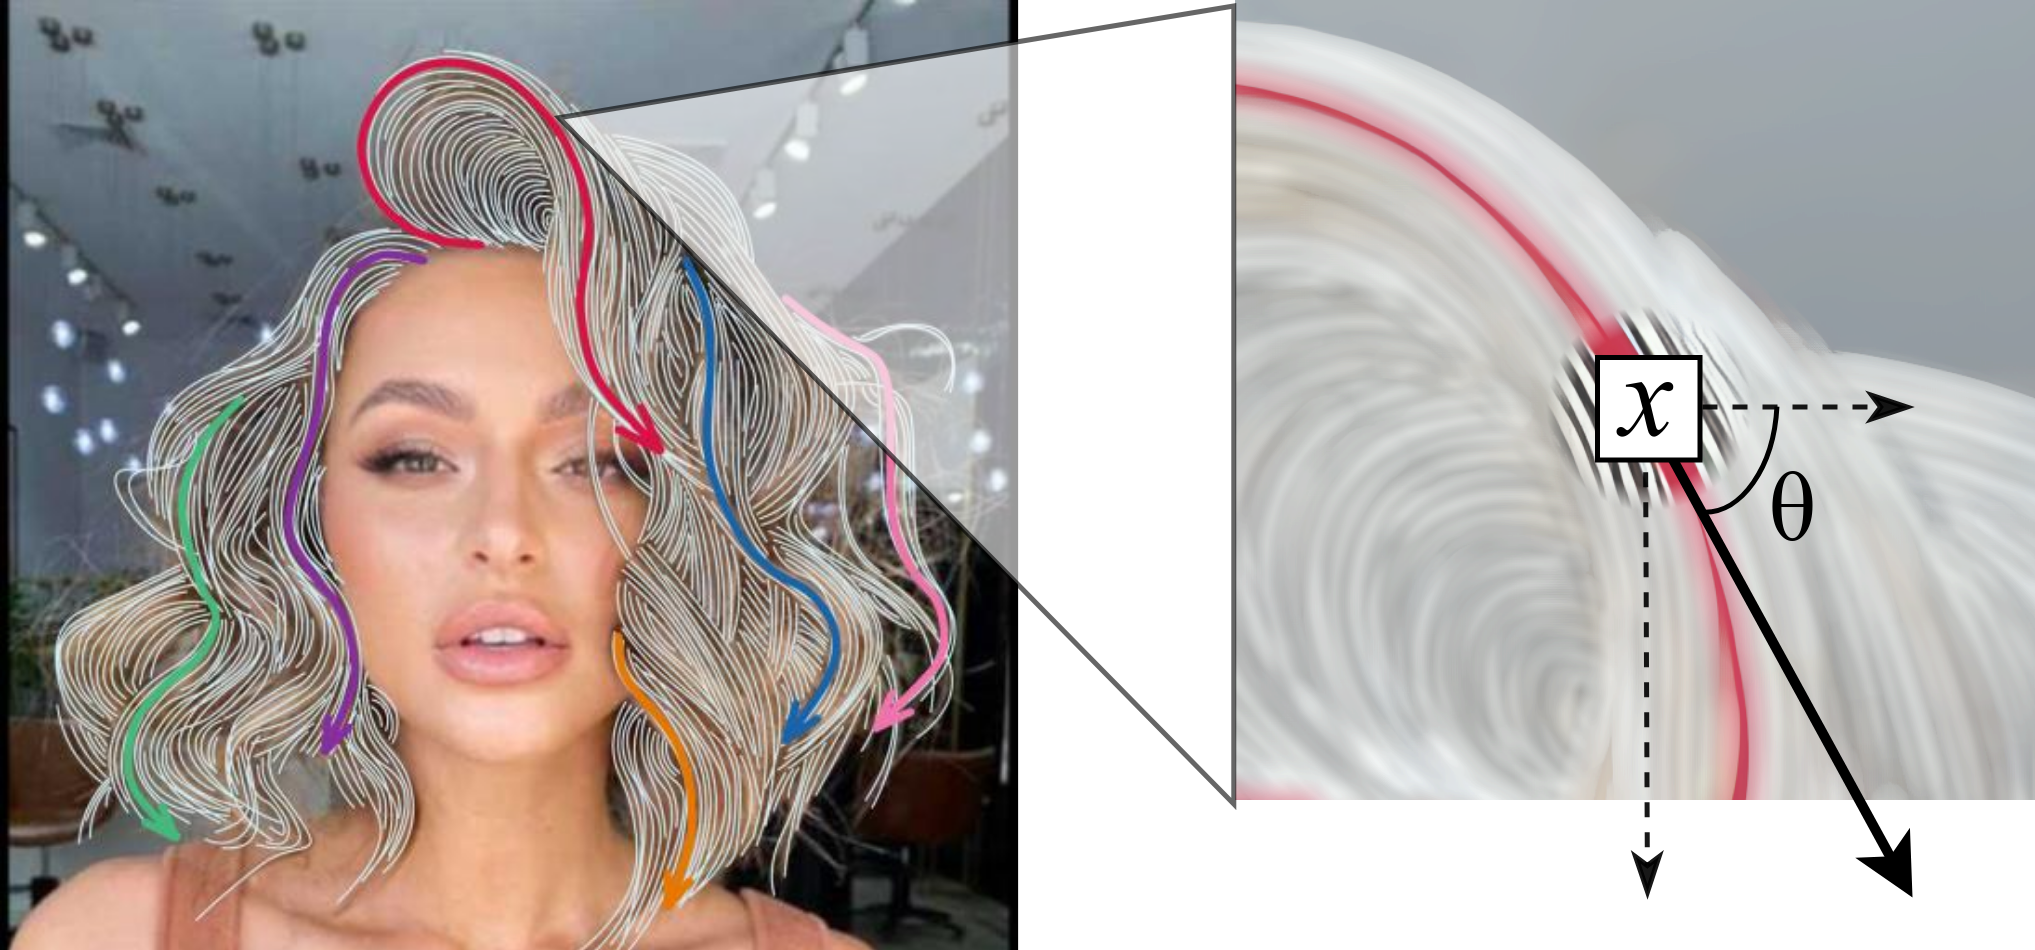
\includegraphics[width=0.45\textwidth]{assets/figures/method/hisa/o_2d.png}
        \caption{Visualization of $\mathbf{O}_{\mathrm{2D}}(x)$, where 
        $\mathbf{O}_{\mathrm{2D}}(x) = \begin{bmatrix}\cos(\theta) \\ -\sin(\theta)\end{bmatrix}$.}
        \label{fig:o_2d_example}
    \end{figure}
\end{frame}

%---------------------------------------------------------
\begin{frame}[t]{HairStep Representation -- Depth Map}
    The \emph{Depth Map} $\mathbf{D} \in \mathbb{R}^{W \times H \times 1}$ defines
    relative depth differences among hair strands.

    \begin{itemize}
        \item Each pixel $\mathbf{D}(x) \in [0, 1]$:
        \begin{itemize}
            \item $\mathbf{D}(x) = 0$: Farthest from the camera (or background, where $\mathbf{M}(x)=0$).
            \item $\mathbf{D}(x) = 1$: Closest to the camera.
        \end{itemize}
    \end{itemize}  % <-- end the outer itemize before starting the figure environment

    \begin{figure}[t]
        \centering
        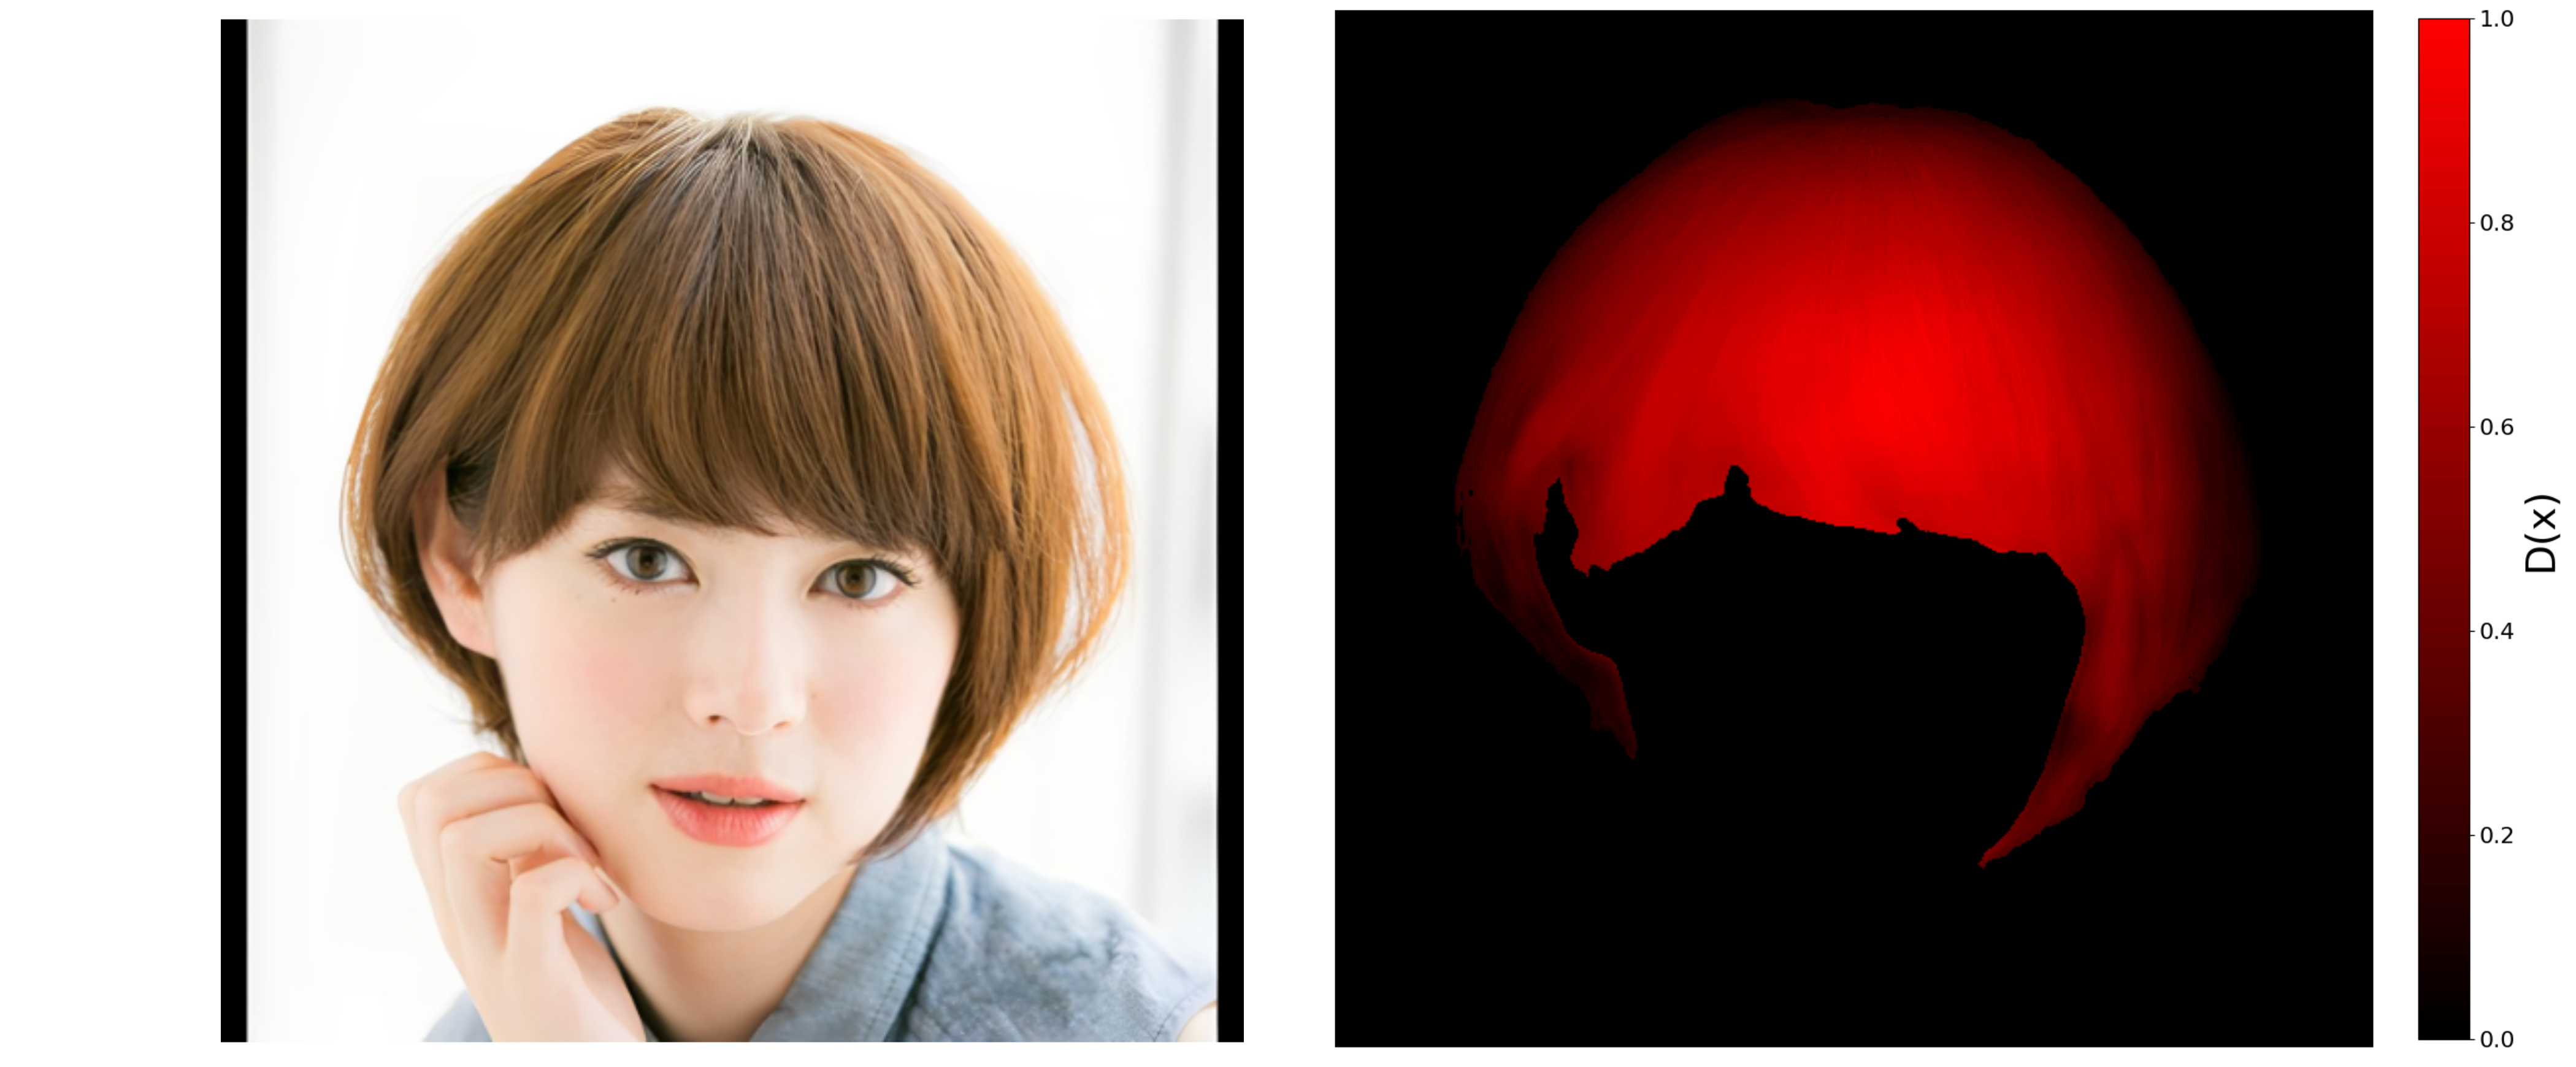
\includegraphics[width=0.55\textwidth]{assets/figures/method/depth-map/depth-map.png}
        \caption{Example of the depth map $\mathbf{D}(x)$.}
        \label{fig:depth_map_example}
    \end{figure}
\end{frame}

%---------------------------------------------------------
\subsection{Overview}
%---------------------------------------------------------

\begin{frame}{Overview}
    \begin{figure}[t]
        \centering
        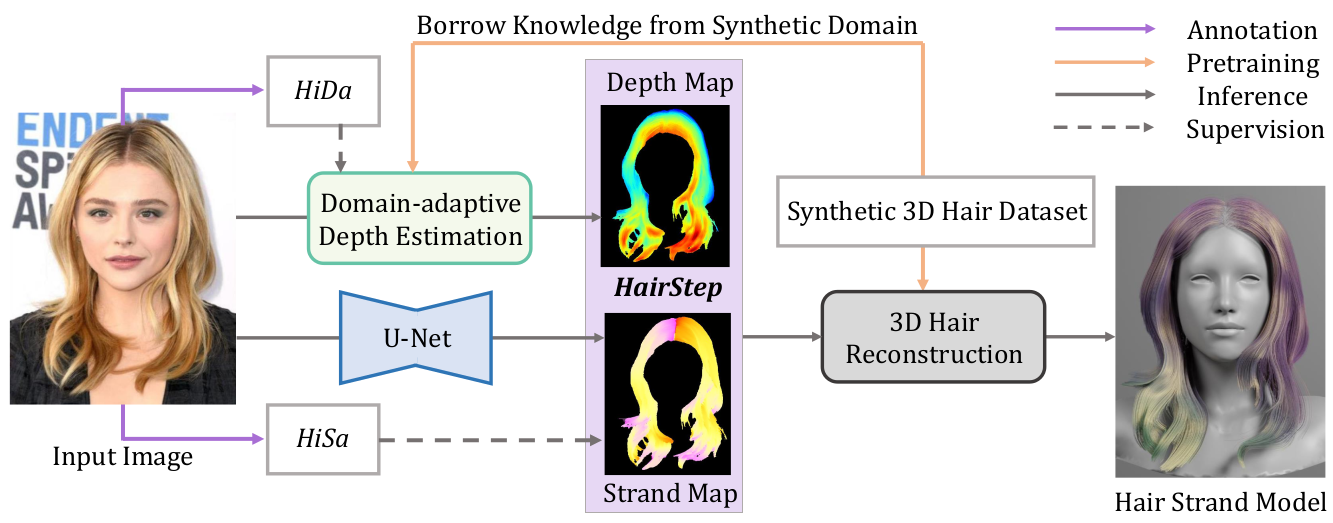
\includegraphics[width=0.95\textwidth]{assets/figures/method/overview.png}
        \caption{The pipeline of single-view 3D hair reconstruction using \textit{HairStep}.}
        \label{fig:overview}
    \end{figure}
\end{frame}

%---------------------------------------------------------
\begin{frame}[t]{Overview}
    The pipeline has three main components:
    \begin{itemize}
        \item \textbf{Strand Map Extraction \& Prediction:} 
        \begin{itemize}
            \item Extract strand maps from real images using the \textit{HiSa} dataset.
        \end{itemize}
        \item \textbf{Domain-Adaptive Depth Estimation:}
        \begin{itemize}
            \item Estimate relative depth from real images using the \textit{HiDa} dataset.
            \item Weakly supervise depth estimation using synthetic data.
        \end{itemize}
        \item \textbf{3D Hair Reconstruction:}
        \begin{itemize}
            \item Reconstruct 3D hair strands from the predicted strand and depth maps.
        \end{itemize}
    \end{itemize}
\end{frame}

%---------------------------------------------------------
\subsection{Strand Map Extraction \& Prediction}
%---------------------------------------------------------

\begin{frame}[t]{Strand Map Extraction}
    Extracting strand maps is crucial for learning-based 3D hair modeling.
    \begin{itemize}
        \item \textbf{Synthetic}: Use rendering techniques (e.g.\cite{liu2019softras}).
        \item \textbf{Real}: Use a U-Net trained on the \textit{HiSa} dataset.
    \end{itemize}
\end{frame}

%---------------------------------------------------------
\begin{frame}[t]{HiSa Dataset}
    The \emph{HiSa} dataset provides strand maps for real images.

    \begin{itemize}
        \item \textbf{Collection:} 1,250 portrait images.
        \item \textbf{Annotation Process:}
        \begin{itemize}
            \item Artists draw directional vector curves from the hair roots to the hair ends.
            \item Vector strokes are colored by the definition of Eq.~\ref{eq:strand_map}.
            \item Colored strokes are interpolated to form the strand map.
        \end{itemize}
        \item \textbf{Statistics:}
        \begin{itemize}
            \item On average, 300 strokes per portrait is annotated.
        \end{itemize}
    \end{itemize}
\end{frame}

%---------------------------------------------------------
\begin{frame}{HiSa Dataset (Visualization)}
    \begin{figure}[t]
        \centering
        \includegraphics[width=0.95\textwidth]{assets/figures/method/hisa/hisa.png}
        \caption{Strand maps extraction steps:
        (a) Portrait image, (b) Annotated vector strokes, (c) Colored strokes, (d) Strand map.}
        \label{fig:hisa}
    \end{figure}
\end{frame}

%---------------------------------------------------------
\begin{frame}{Strand Map Prediction}
    \begin{figure}[t]
        \centering
        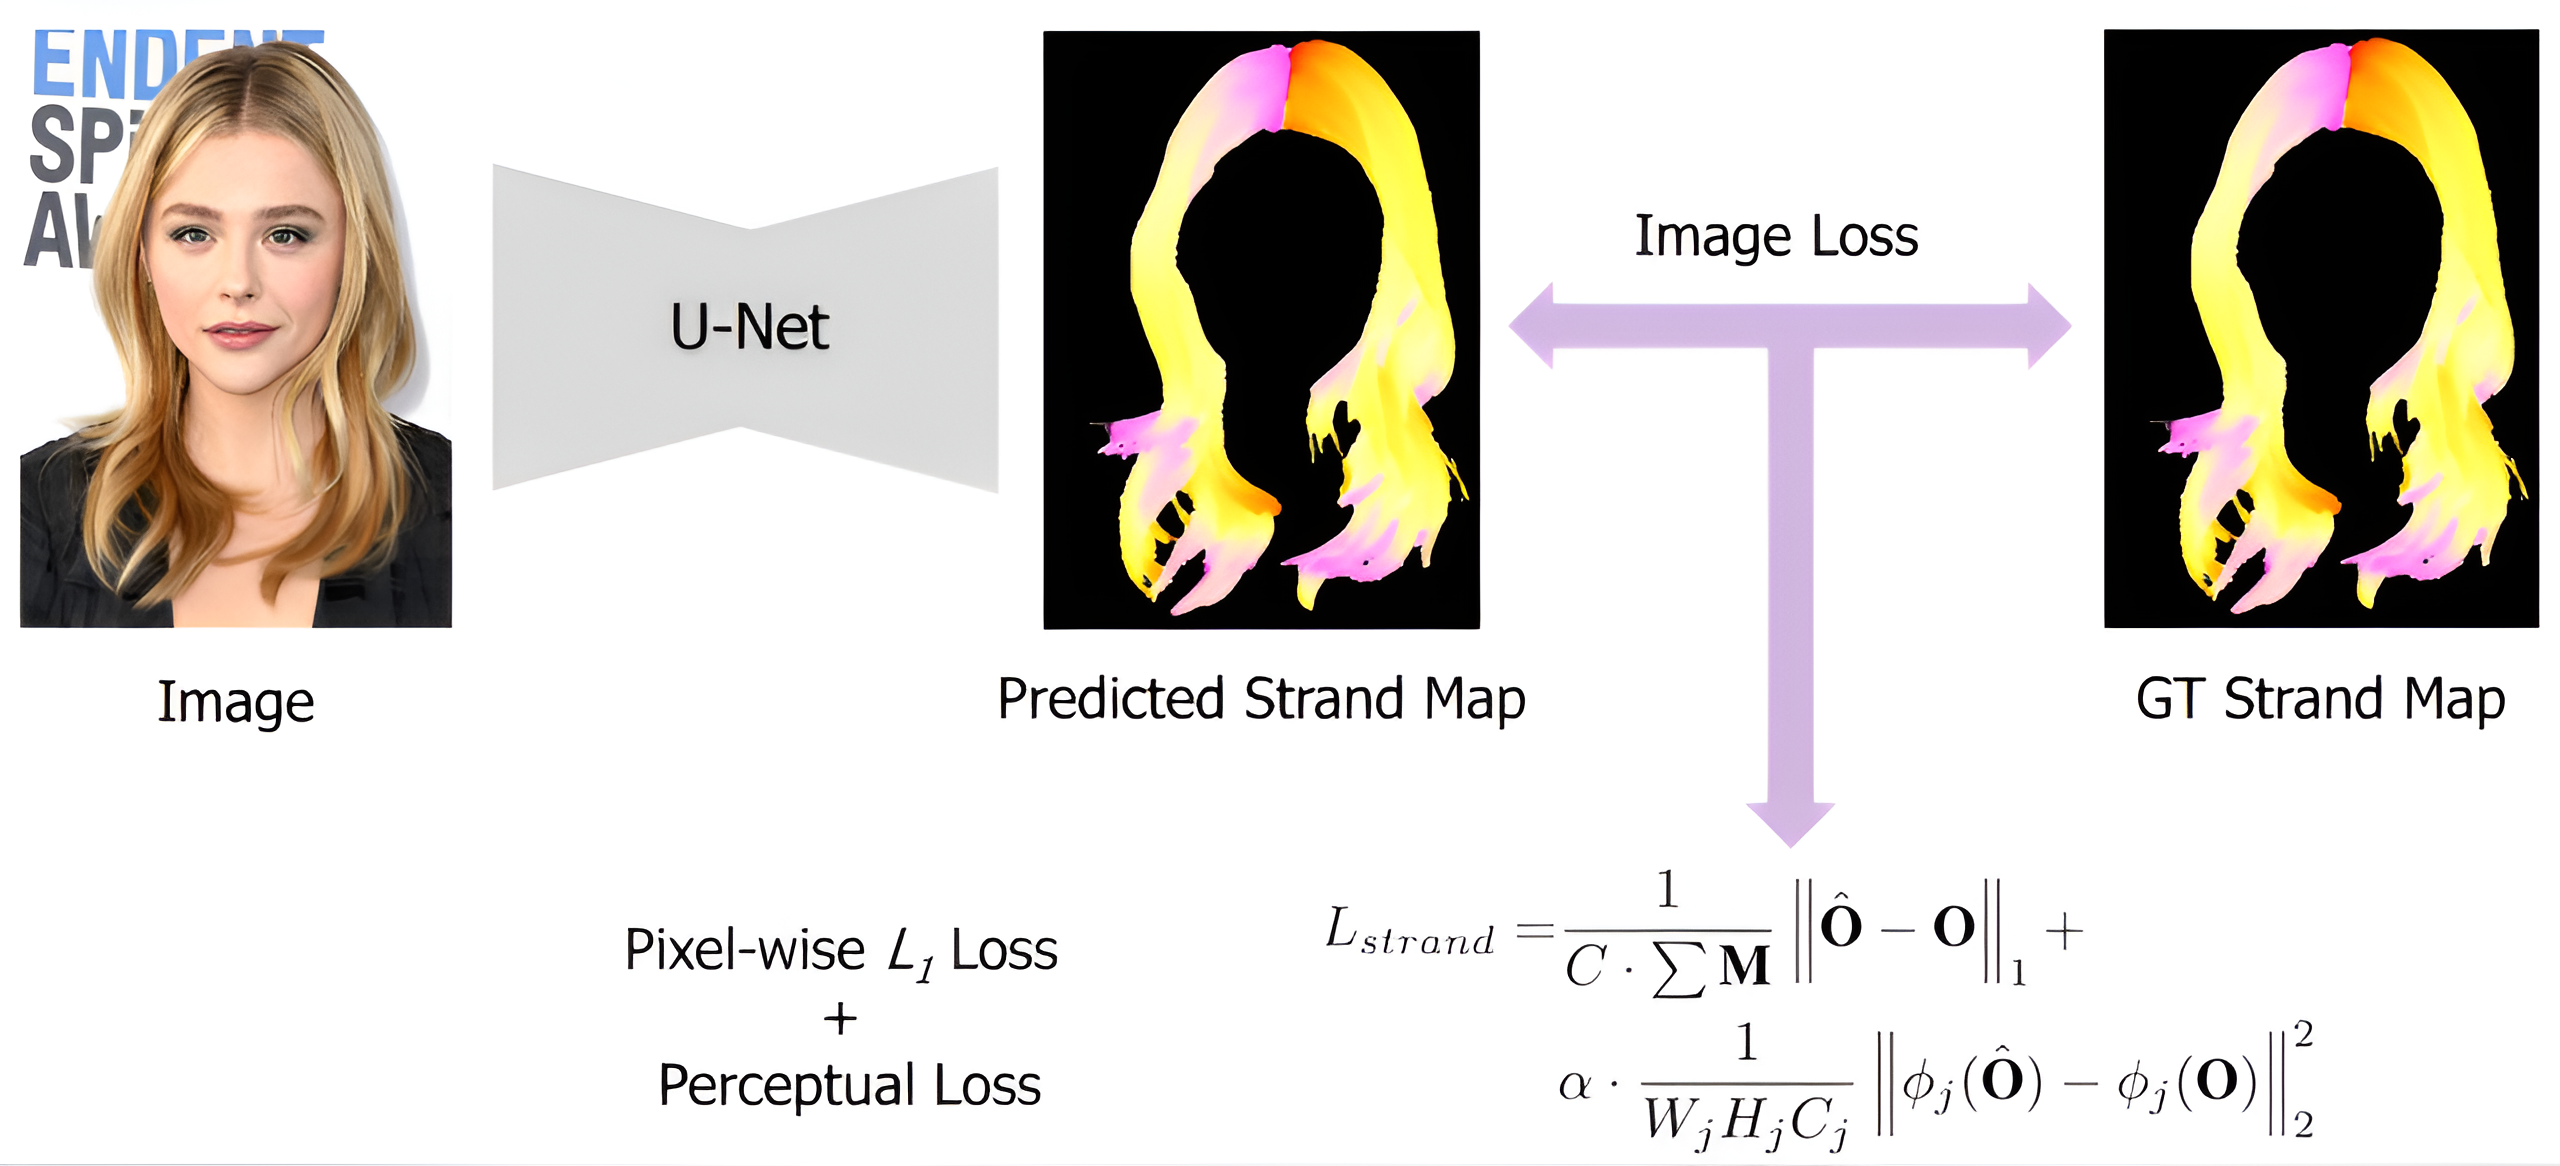
\includegraphics[width=0.95\textwidth]{assets/figures/method/strand/prediction.png}
        \caption{Example pipeline for strand map prediction.}
        \label{fig:strand-map-prediction}
    \end{figure}
\end{frame}

%---------------------------------------------------------
\subsection{Depth Estimation and HiDa Dataset}
%---------------------------------------------------------

\begin{frame}{Relative Depth Estimation}
    Inspired by the depth-in-the-wild approach~\cite{Zhou2018SingleViewHR}, relative depth estimation serves as a weak supervision signal.
    \begin{figure}[t]
        \centering
        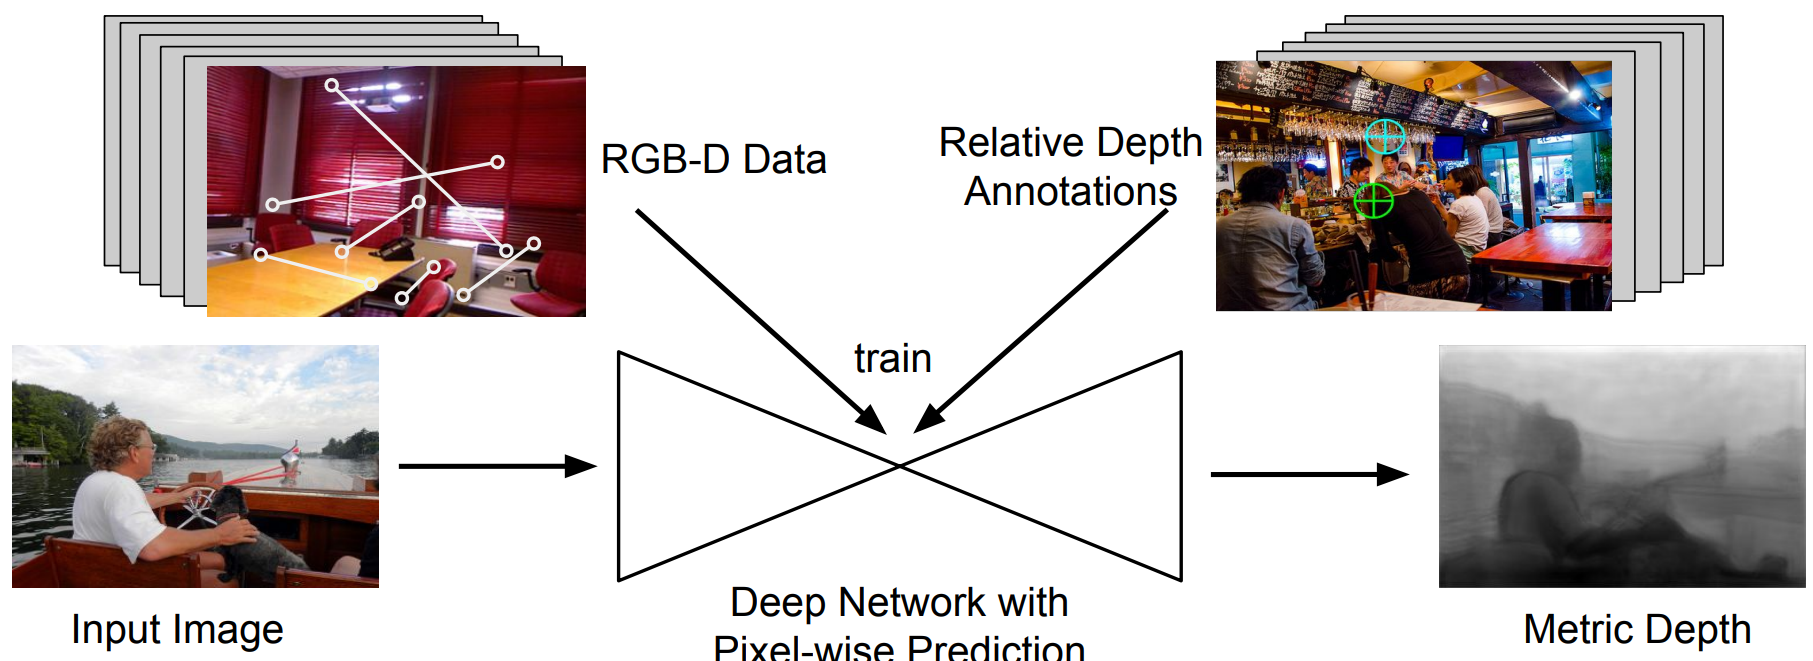
\includegraphics[width=0.85\textwidth]{assets/figures/method/depth/depth-in-the-wild.png}
        \caption{Overview of the depth-in-the-wild pipeline.}
        \label{fig:depth_in_the_wild}
    \end{figure}
\end{frame}

%---------------------------------------------------------
\begin{frame}[t]{HiDa Dataset}
    The \emph{HiDa} dataset provides relative depth annotations for hair regions in real images.

    \begin{itemize}
        \item \textbf{Collection:} 1,250 portrait images (the same as \textit{HiSa}).
        \item \textbf{Annotation Process:}
        \begin{itemize}
            \item Generate super-pixels within the hair region.
            \item Sample pixel pairs from adjacent super-pixels.
            \item Show each pair on the portrait and ask annotators which point is closer.
        \end{itemize}
        \item \textbf{Statistics:}
        \begin{itemize}
            \item On average, 140 pairs per portrait.
            \item 129,079 annotated pixel pairs in total.
        \end{itemize}
    \end{itemize}
\end{frame}


%---------------------------------------------------------
\begin{frame}[t]{HiDa Dataset (Visualization)}
    \begin{figure}[t]
        \centering
        \includegraphics[width=0.8\textwidth]{assets/figures/method/hida/superpixel.png}
        \caption{Example of super-pixels generated for the HiDa dataset.}
        \label{fig:hida-superpixel}
    \end{figure}
\end{frame}

%---------------------------------------------------------
\begin{frame}{Domain-Adaptive Depth Estimation}
    \begin{figure}[t]
        \centering
        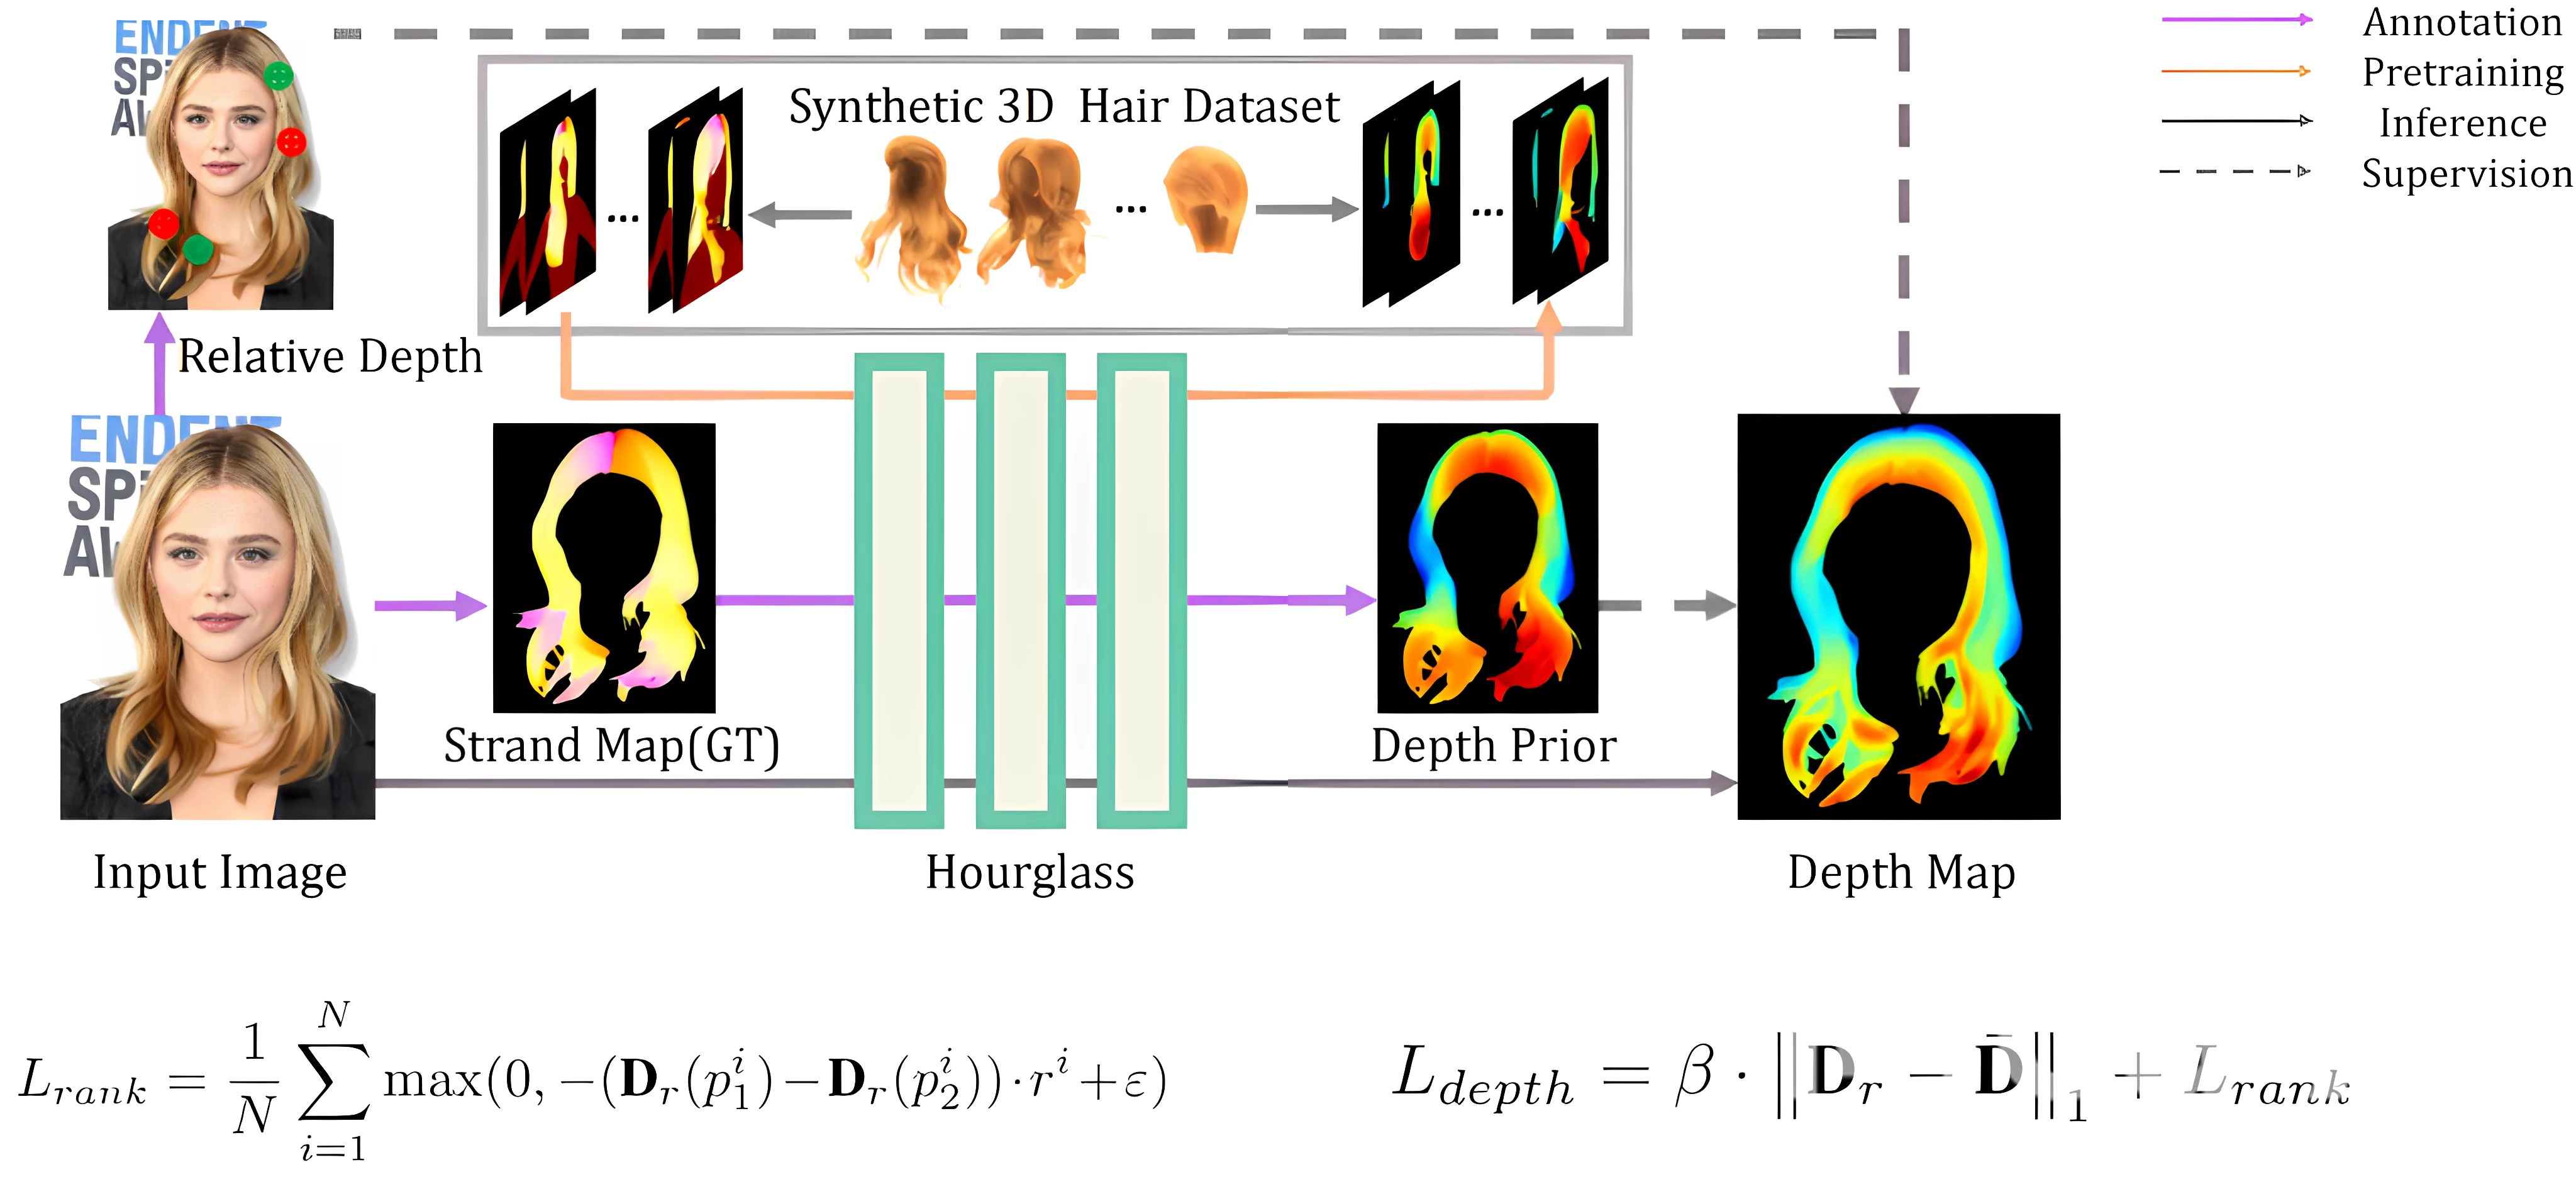
\includegraphics[width=0.9\textwidth]{assets/figures/method/depth/pipeline.png}
        \caption{Overview of the domain-adaptive depth estimation approach.}
        \label{fig:depth_estimation_overview}
    \end{figure}
\end{frame}

%---------------------------------------------------------
\begin{frame}{Depth Estimation}
    We use an \emph{Hourglass} network to predict depth maps from input images. 
    A margin-based ranking loss is applied for relative depth estimation.
    \begin{figure}[t]
        \centering
        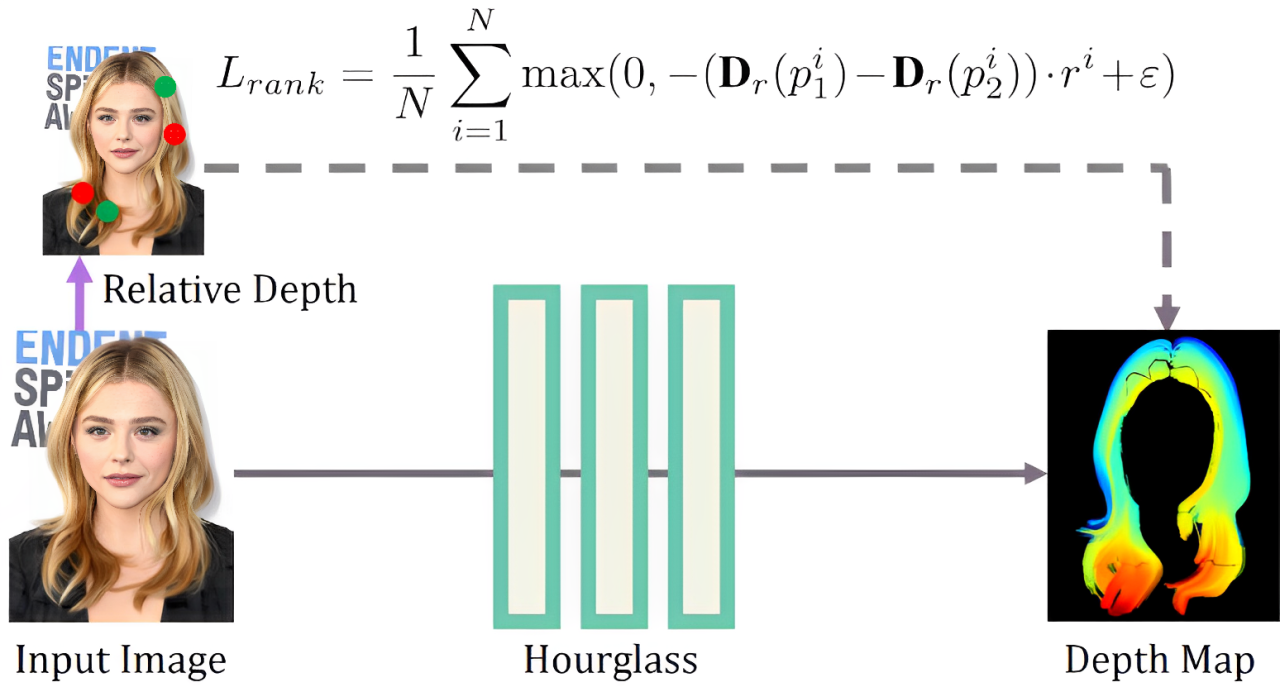
\includegraphics[width=0.6\textwidth]{assets/figures/method/depth/hourglass.png}
        \caption{Each pair $(p^i_1, p^i_2)$ forms the $i$-th annotated pair; $r^i=1$ if $p^i_1$ is closer, $r^i=-1$ otherwise.}
        \label{fig:hourglass_depth}
    \end{figure}
\end{frame}

%---------------------------------------------------------
\begin{frame}[t]{Depth Estimation Challenges}
    Training with only ordinal labels can introduce ambiguity and artifacts in depth prediction, resulting in noisy or coarse 3D hair models.
    \vspace{0.5em}
    \begin{figure}[t]
        \centering
        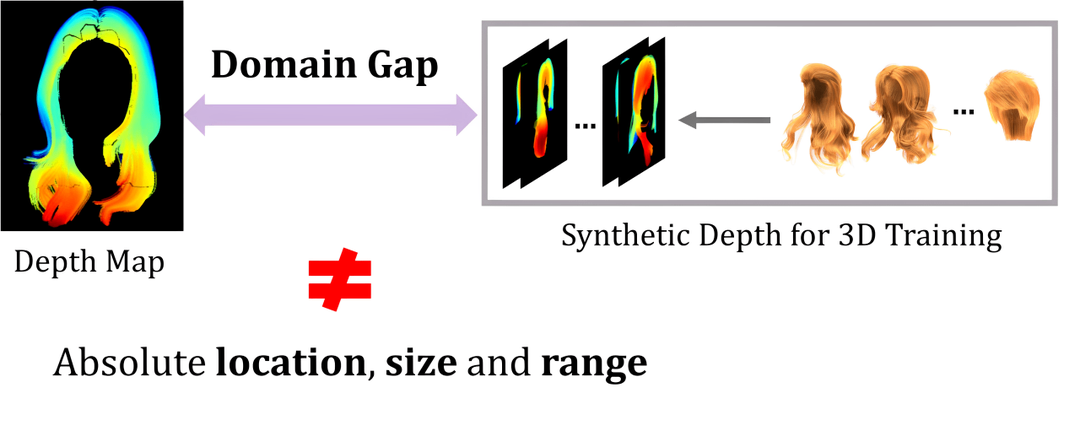
\includegraphics[width=0.6\textwidth]{assets/figures/method/depth/domain-gap.png}
        \caption{Domain gaps and artifacts in predicted depth from ordinal labels.}
        \label{fig:domain_gap}
    \end{figure}
\end{frame}

%---------------------------------------------------------
\begin{frame}[t]{Domain-Adaptive Depth Estimation}
    To mitigate artifacts, a domain-adaptive depth estimation pipeline refines depth predictions using synthetic data:
    \begin{itemize}
        \item \textbf{Pre-training} a Hourglass network \texttt{Depth\_syn} on synthetic data:
        \begin{itemize}
            \item Input: Ground-truth strand map.
            \item Output: Depth map $\bar{\mathbf{D}}$.
            \item Loss: $L_1$ loss on $\bar{\mathbf{D}}$.
        \end{itemize}
        \item \textbf{Training} a Hourglass network \texttt{Depth\_r} on real data:
        \begin{itemize}
            \item Input: Real images + ground-truth strand map.
            \item Output: Depth map $\mathbf{D}_r$.
            \item Supervision: Depth prior $\bar{\mathbf{D}}$ from \texttt{Depth\_syn}.
            \item Final Loss: $L_{\text{depth}} = \beta \|\mathbf{D}_r - \bar{\mathbf{D}}\|_1 + L_{\text{rank}}$.
        \end{itemize}
    \end{itemize}
\end{frame}

%---------------------------------------------------------
\subsection{Single-View 3D Hair Modeling}
%---------------------------------------------------------

\begin{frame}[t]{Single-View 3D Hair Modeling}
    \begin{figure}[t]
        \centering
        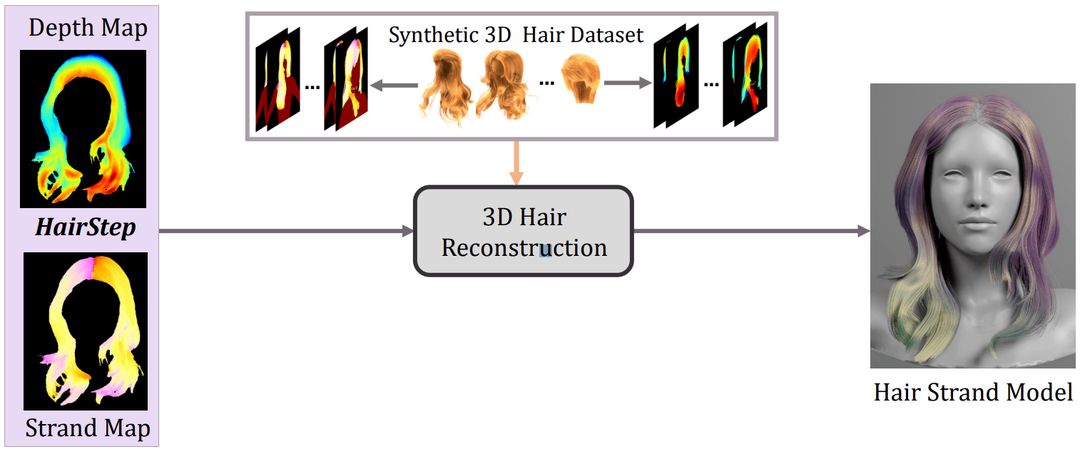
\includegraphics[width=0.9\textwidth]{assets/figures/method/reconstruction.png}
        \caption{Pipeline for single-view 3D hair modeling using \emph{HairStep}.}
        \label{fig:single_view_3d_hair_modeling}
    \end{figure}
\end{frame}

%---------------------------------------------------------
\begin{frame}[t]{Single-View 3D Hair Modeling Details}
    \textbf{Objective:} Reconstruct strand-level 3D hair from a \emph{single-view} portrait image via the \emph{HairStep} representation $\{\mathbf{O}, \mathbf{D}\}$.
    \begin{itemize}
        \item \textbf{Key Idea:} Convert HairStep into \emph{implicit fields} encoding 3D hair geometry.
        \item \textbf{Two Main Stages}:
        \begin{itemize}
            \item \textbf{Implicit Representation:} Predict occupancy and orientation fields in a canonical head space.
            \item \textbf{Strand Generation:} Convert those fields into explicit 3D hair strands.
        \end{itemize}
    \end{itemize}
\end{frame}

%---------------------------------------------------------
\begin{frame}[t]{Implicit 3D Hair Representation}
    \textbf{Why Implicit Fields?}
    \begin{itemize}
        \item Flexible, memory-efficient for complex volumetric structures like hair.
        \item Smoothly captures continuous geometry and orientations without enumerating every strand.
    \end{itemize}

    \textbf{Following NeuralHDHair~\cite{wu2022neuralhdhair}, define:}
    \begin{itemize}
        \item \textbf{Occupancy Field} $f_{\text{occ}}(v) \in [0,1]$:
        \begin{itemize}
            \item Indicates inside vs.\ outside the hair volume.
            \item $f_{\text{occ}}(v) = 1$ if $v$ is inside hair; $0$ otherwise.
        \end{itemize}
        \item \textbf{Orientation Field} $f_{\text{orient}}(v) \in \mathbb{R}^3$:
        \begin{itemize}
            \item Unit vector of local hair-growth direction inside hair volume.
            \item Zero vector outside.
        \end{itemize}
    \end{itemize}
\end{frame}

%---------------------------------------------------------
\begin{frame}[t]{Neural Network Prediction (NeuralHDHair)}
    \textbf{NeuralHDHair*} \emph{(adapted from~\cite{wu2022neuralhdhair})}
    \begin{itemize}
        \item \textbf{Input:} Strand map $\mathbf{O}$ and depth map $\mathbf{D}$ (4-channel input including hair mask).
        \item \textbf{Output:} Implicit occupancy $f_{\text{occ}}(\mathbf{x})$ and orientation $f_{\text{orient}}(\mathbf{x})$ fields.
        \item \textbf{Modifications:}
        \begin{itemize}
            \item \emph{No Luminance Map}: Reduces domain gap from lighting differences.
            \item \emph{Omit GrowingNet}: Focus on reconstruction quality using direct strand-growing from implicit fields.
        \end{itemize}
    \end{itemize}
\end{frame}

%---------------------------------------------------------
\begin{frame}[t]{Hair Strand Generation}
    After predicting the implicit fields, hair strands are generated following DeepSketchHair~\cite{shen2020deepsketchhair}:
    \begin{itemize}
        \item \textbf{Initialization:}
        \begin{itemize}
            \item Place hair roots on a standard scalp model.
        \end{itemize}
        \item \textbf{Strand Growing:}
        \begin{itemize}
            \item From each root, follow $f_{\text{orient}}$.
            \item Stop when $f_{\text{occ}} = 0$ or reaching max length.
        \end{itemize}
        \item \textbf{Result:}
        \begin{itemize}
            \item A dense set of 3D hair strands ($\sim$10K strands) replicating the input hairstyle.
        \end{itemize}
    \end{itemize}
\end{frame}
